%%%%%%%%%%%%%%%%%%%%%%%%%%%%%%%%%%%%%%%%%%%%%%%%%%%%%%%%%%%%%%%
%
% Welcome to Overleaf --- just edit your LaTeX on the left,
% and we'll compile it for you on the right. If you open the
% 'Share' menu, you can invite other users to edit at the same
% time. See www.overleaf.com/learn for more info. Enjoy!
%
%%%%%%%%%%%%%%%%%%%%%%%%%%%%%%%%%%%%%%%%%%%%%%%%%%%%%%%%%%%%%%%
\documentclass{beamer}

\usetheme{Madrid}
\usecolortheme{lily}
\addtobeamertemplate{footnote}{}{\vspace{2ex}}

\usepackage{amsmath}
\usepackage{amssymb}
\usepackage{color}
\usepackage{listings}
\usepackage{clrscode3e}
\usepackage{multicol}
\usepackage{tikz}

\definecolor{codegreen}{HTML}{237e02}
\definecolor{codegray}{rgb}{0.5,0.5,0.5}
\definecolor{codepurple}{HTML}{8F4673}
\definecolor{codebrown}{HTML}{ce9178}
\definecolor{codecyan}{HTML}{098658}
\lstdefinestyle{pythonstyle}{
    commentstyle=\color{codegreen},
    keywordstyle=\color{codepurple},
    numberstyle=\tiny\color{codegray},
    stringstyle=\color{codebrown},
    basicstyle=\ttfamily\small,
    breakatwhitespace=false,         
    breaklines=true,                 
    captionpos=b,                    
    keepspaces=true,                 
    numbersep=5pt,                  
    showspaces=false,                
    showstringspaces=false,
    showtabs=false,
    tabsize=2
}
\def\And{\text{ AND }}
\def\Or{\text{ OR }}
\def\Xor{\text{ XOR }}
\def\Implies{\text{ IMPLIES }}
\def\Iff{\text{ IFF }}
\def\Not{\text{NOT}}
\def\R{\mathbb{R}}
\def\N{\mathbb{N}}
\lstset{style=pythonstyle}

\setlength{\parskip}{1em}

%Information to be included in the title page:
\title{Format for Efficient Storage of Homology Relations}
\subtitle{Week 7 Report: Interval Labeling Index}
\author{Kevin Gao}
\institute{University of Toronto}

\begin{document}

\frame{\titlepage}

\AtBeginSection[]
{
    \begin{frame}
    \frametitle{Outlines}
    \tableofcontents[currentsection]
    \end{frame}
}

\section{Idea of Interval-based Indexing}

\begin{frame}{Idea of Interval-based Indexing}
    The interval index uses an interval-based labeling scheme. We begin by assigning every leaf $x$ a unique label, denoted $\id{label}(x)$. This is maintained in two hash tables: one that maps leaf to label, and another one that maps label to leaf. A label to a leaf is called a \textbf{leaf label}.

    Let $v$ be an internal vertex, and suppose that $v$ has a set of leaves in the subtree rooted at $v$, say $L$, with labels $L' = \{\id{label}(x) \mid x \in L\}$. Then, we assign $v$ the label $\min\{L'\}\$\max\{L'\}$ where $\$$ is a delimiter. A label to an internal node is called an \textbf{internal label}. Given an internal label $l$, we use $l_1$ to denote the first part of the label (the portion before the delimiter), and use $l_2$ to denote the second part of the label (the portion after the delimiter). For clearity, we use $(l_1,l_2)$ instead of $l_1 \$ l_2$ in future discussions.

    An interval labeling can be constructed by first assigning leaf labels and iteratively updating the internal nodes on the leaf-to-root path for each leaf.
\end{frame}

\begin{frame}{Example of Interval-based Index}
    \begin{tikzpicture}
        [
            level 1/.style = {sibling distance = 4cm},
            level 2/.style = {sibling distance = 2.5cm}
        ]
         
        \node {(0,3)}
            child {
                node {(0,1)}
                child {node {0}}
                child {node {1}}
            } 
            child {
                node {(2,3)}
                child {
                    node {(2,2)}
                    child {node {2}}
                }
                child {node {3}}
            };
        \end{tikzpicture}

        Leaves are labeled sequentially from left to right. Internal nodes are labeled based on the minimum leaf label and maximum label in the subtree rooted at that internal node.
\end{frame}

\section{Querying the Index}

\begin{frame}{How to Query the Interval Index}
    Given two vertices and their corresponding labels, we can determine whether a vertex is an ancestor of another vertex via a range query of interval containment of their labels. A leaf label of value $x$ can be thought as the interval $[x,x]$.

    Given two leaves labeled $x$ and $y$, we find the LCA by finding the shortest interval containing both $x$ and $y$. This gives us the \textit{lowest} common ancestor because the size of the interval is non-decreasing as we traverse from a leaf to root.

    Given a gene represented as a leaf labeled $x$, in order to find all orthologs of the gene, we find all intervals containing $x$ that are labels to a speciation node. We also remove the intervals (internal nodes) that are visited. After this, suppose we have non-overlapping intervals $S = \{[a,b],\; [c,d],\ldots\}$. Then, clearly, all the leaves with integer labels from $a$ to $b$ and so on are orthologs of the leaf labeled $x$.
\end{frame}

\begin{frame}{Key Observations}
    \textit{Observation 1}: Let $x$ be a leaf in a tree. There is a unique path of length $\id{depth}(x)$ from $x$ to the root.

    \textit{Observation 2}: Let $x$ be a leaf in a tree and let $P = x \to \cdots \to r$ be the unique path from $x$ to the root $r$. Every internal node on this path $P$ including $r$ is labeled with an interval that contains $x$.

    \textit{Observation 3}: There are exactly $\id{depth}(x)$ internal nodes labeled with an interval that contains $x$.

    \textit{Observation 4}: Let $a$ be an internal node, and let $b$ be the immediate parent of $a$. Then, the interval represented by $a$ is contained in the interval represented by $b$.
\end{frame}

\begin{frame}{More on Query}
    Consider the example tree. Speciation nodes are colored {\color{blue}blue}, and duplication nodes are colored {\color{red}red}.

    \begin{tikzpicture}
        [
            level 1/.style = {sibling distance = 4cm},
            level 2/.style = {sibling distance = 2.5cm}
        ]
         
        \node {\textcolor{blue}{(0,4)}}
            child {
                node {\textcolor{red}{(0,1)}}
                child {node {0}}
                child {node {1}}
            } 
            child {
                node {\textcolor{red}{(2,4)}}
                child {
                    node {\textcolor{blue}{(2,3)}}
                    child {node {2}}
                    child {node {3}}
                }
                child {node {4}}
            };
    \end{tikzpicture}
\end{frame}

\begin{frame}{More on Query}
    Suppose we want to find all orthologs of the gene labeled `2'. We consider all internal nodes on the unique leaf-to-root path originating from `2'. The intervals are: (2,3), (2,4), (0,4). We maintain two arrays: $\id{orthologs}$ and $\id{visited}$.

    $\id{orthologs}$ stores the orthologs discovered. $\id{visited}$ stores the intervals that are already visited on the path.

    \begin{itemize}
        \item \textcolor{blue}{(2, 3)}: speciation node, $\id{visited} = []$, $\id{orthologs} = []$
        \item \textcolor{red}{(2, 4)}: duplication node, \textbf{skip}, $\id{visited} = [(2,3)]$, $\id{orthologs} = [2,3]$
        \item \textcolor{blue}{(0, 4)}: speciation node, $[(0,1)]$ after excluding the visited intervals, $\id{visited} = [(2,3),\, (2,4)]$, $\id{orthologs} = [2,3]$
        \item Result: $\id{visited} = [(2,3),\,(2,4),\,(0,1)]$, $\id{orthologs} = [2,3,0,1]$
    \end{itemize}
\end{frame}

\section{Maintaining the Information}

\begin{frame}{All Intervals Covering a Certain Point}
    One of the queries central to our algorithm is the problem of finding all intervals covering a point given a query point and a set of intervals to query from.

    Based on Observation 3, with our labeling scheme, all the intervals containing a point $x$ are labels of the internal nodes on the leaf-to-root path from the leaf labeled with $x$. We need to at least visit $\id{depth}(x)$ many nodes to collect all intervals containing $x$.

    If we have the tree structure parsed from the input residing in the memory with efficient random access, we can traverse the tree starting from the node labeled with our query label $x$. This takes precisely $\id{depth}(x)$ node visits.

    Otherwise, we can construct an interval tree.
\end{frame}

\begin{frame}{Interval Tree}
    \textbf{Interval tree} (centered interval tree) is a tree data structure for storing intervals and efficient interval queries. As we will discuss later, interval tree takes $O(n \log n)$ time to construct, and query (point query or interval query) takes $O(\log n)$ using an algorithm resembling binary search. $n$ is the number of intervals, which in the context of our problem is the number of internal nodes in the original tree.

    Given a set of intervals $S$, the interval tree for $S$ stores the median $x_{mid}$, along with the set of intervals overlapping with $x_{mid}$ at the root. The left subtree of the root is an interval tree for all intervals whose right endpoint is less than $x_{mid}$. The right subtree is an interval tree for all intervals whose left endpoint is larger than $x_{mid}$.
\end{frame}

\section{Storing the Interval Index}

\begin{frame}{Data to Keep Track of}
    There are a few fields that we need to keep track of:
    \begin{itemize}
        \item Bijection between node and labels: use hashing?
        \item List of all speciation node labels
        \item List of all duplication node labels
    \end{itemize}
    With our current implementation, they are stored directly within the memory. But for our data format, we will encode these fields into a separate binary index file. Storing the index in a separate file would increase interoperability.
\end{frame}

\section{Benchmark Results in Python}

\begin{frame}{Benchmark Result}
    Benchmarks are done on trees of various sizes. Compared to non-indexed methods, we can perform on average 2 to 3 times more operations per second.

    \begin{figure}[htbp]
        \centering
        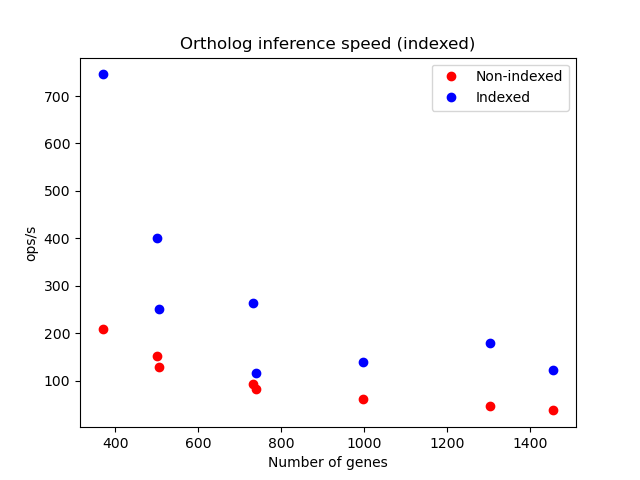
\includegraphics[width=0.5\linewidth]{res/ortholog_inference_performance_number_indexed.png}
        \caption{Operations per second on different trees.}
        \label{fig:ops-per-sec-plot}
    \end{figure}
\end{frame}

\begin{frame}{Other Considerations}
    Skewed trees and especially trees with a lot of speciation nodes but relatively fews duplication nodes (and vice versa) has visible performance drop compared to other trees.
    \begin{figure}[htbp]
        \centering
        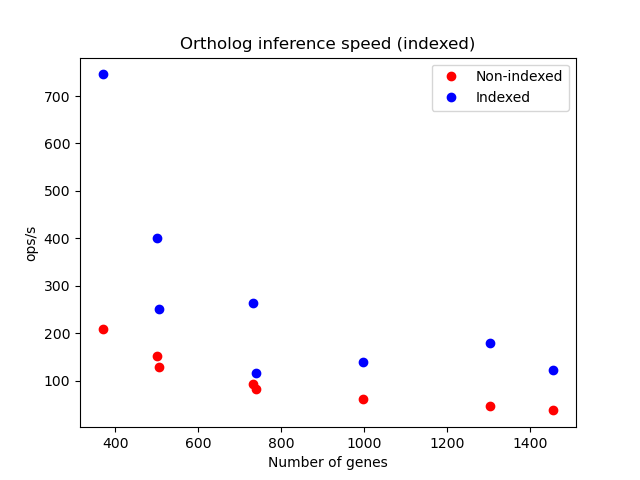
\includegraphics[width=0.5\linewidth]{res/ortholog_inference_performance_number_indexed.png}
        \caption{Two trees of size 500 but very different number of speciation nodes shows performance fluctuation depending on number of speciation/duplication.}
        \label{fig:ops-per-sec-plot-skew}
    \end{figure}
\end{frame}

\begin{frame}{The Whole Picture}
    \begin{figure}[htbp]
        \centering
        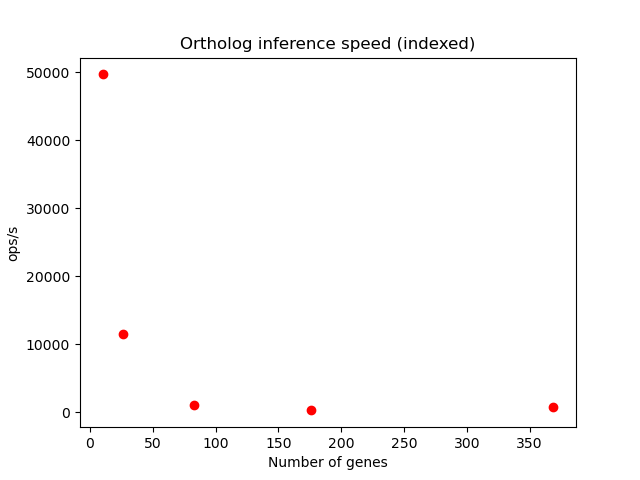
\includegraphics[width=0.45\linewidth]{res/ortholog_inference_performance_number_indexed copy.png}
        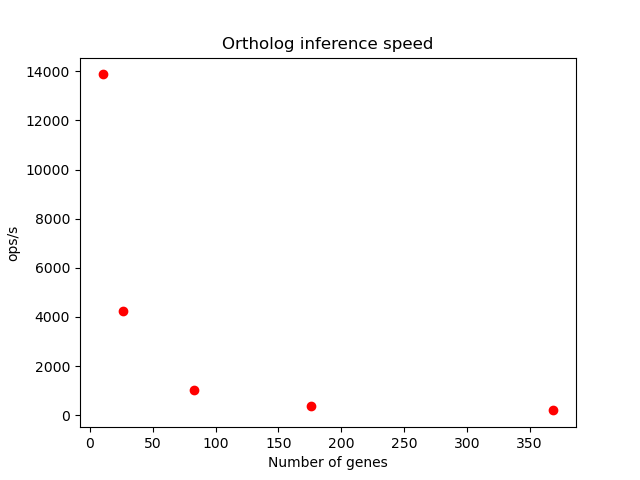
\includegraphics[width=0.45\linewidth]{res/ortholog_inference_performance_number.png}
    \end{figure}
\end{frame}

\section{References}

\begin{frame}
    \scriptsize

    Zhang, J., Lovette, K.: XimpleWare W3C Position Paper. In: W3C Workshop on Binary Interchange of XML Information Item Sets (2003)
\end{frame}

\end{document}